
%(BEGIN_QUESTION)
% Copyright 2006, Tony R. Kuphaldt, released under the Creative Commons Attribution License (v 1.0)
% This means you may do almost anything with this work of mine, so long as you give me proper credit

A ``smart'' differential pressure transmitter is configured to measure the differential pressure created by an orifice plate, and also to perform the square-root function necessary to linearize the orifice plate's signal:

$$\includegraphics[width=15.5cm]{i00708x01.eps}$$

Calculate the following:

\begin{itemize}
\item{} Loop current at 350 GPM = \underbar{\hskip 50pt} mA
\vskip 5pt
\item{} Differential pressure at 600 GPM = \underbar{\hskip 50pt} "WC
\end{itemize}

\underbar{file i00708}
%(END_QUESTION)





%(BEGIN_ANSWER)

\begin{itemize}
\item{} Loop current at 350 GPM = \underbar{\bf 9.091} mA
\vskip 5pt
\item{} Differential pressure at 600 GPM = \underbar{\bf 37.19} "WC
\end{itemize}

%(END_ANSWER)





%(BEGIN_NOTES)


%INDEX% Measurement, flow: orifice plate loop calculations

%(END_NOTES)


